\chapter{\label{ch:7}Discussion} 

\graphicspath{{figures/ch7/}}

\minitoc

\section{Summary of findings}

David Colquhoun wrote the following in 1998:
"Distinguishing between effects on binding and effects on conformation change is arguably the fundamental problem of modern molecular studies of receptors.
It is not an easy distinction to make, but unless it can be solved, the interpretation of structure‐function studies is quite likely to be nonsense" \cite{colquhoun_binding_1998}.
A few months earlier, the first crystal structure of an ion channel (the K\textsuperscript{+} channel from \textit{Streptomyces lividans}, KcsA) was published by a team from Roderick MacKinnon's group \cite{doyle_structure_1998}.
While Colquhoun acknowledged that such structures would resolve many questions about the location of ligand binding sites, he emphasised that knowledge of structure does not preclude the search for mechanisms and dynamics: "Structures are static but receptors are not" \cite{colquhoun_binding_1998}.

It took nearly two decades after solving KcsA for structures of the K\ATP{} channel to be resolved through cryo-EM \cite{lee_molecular_2017, martin_anti-diabetic_2017-1, li_structure_2017-1, martin_mechanism_2019-1}.
Impressively, many of the predictions made from detailed electrophysiological experiments and molecular modelling about the inhibitory nucleotide binding site of Kir6.2 were validated by the structures \cite{tucker_molecular_1998, drain_katp_1998, li_i182_2000, cukras_structural_2002, cukras_role_2002, trapp_identification_2003, li_ligand-dependent_2005, antcliff_functional_2005, haider_identification_2007}.
As the structures were solved in complex with ATP and in the absence of lipids, we can assume that they resemble the physiological closed state of the K\ATP{} channel.
The difficulty of obtaining open states of ion channels means that relating the captured structures to the function of K\ATP{} is not trivial, and many open questions remain \cite{puljung_cryo-electron_2018}.

In this thesis, I have aimed to show four things:
\begin{itemize}
\item We can directly measure nucleotide binding to Kir6.2 by site-specifically inserting ANAP at position W311 and measuring its quenching by TNP-ATP.
\item Measuring binding in combination with K\ATP{} channel current inhibition allows us to confirm that an MWC model is able to describe K\ATP{} inhibition by nucleotides.
\item Effects on nucleotide binding and effects on conformational change can be well distinguished by fitting combined binding and inhibition data to an MWC model.
\item SUR1 directly contributes to nucleotide binding to Kir6.2.
\end{itemize}

In doing so, I have built directly on the work of numerous studies using a variety of electrophysiological approaches to provide answers to the above questions.
Where this work differs, and - I believe - adds value, is in two aspects of the approach.
Firstly, while the use of fluorescence to study ligand binding to ion channels is far from novel, the site-specific nature of ANAP incorporation is a development which crucially allows for the separation of nucleotide binding to Kir6.2 from binding to the NBDs of SUR1.
In addition, measuring the quenching of ANAP fluorescence rather than an increase in ligand fluorescence allows us to directly translate our observations into the bound fraction of Kir6.2 subunits, without having to assume that at saturation each subunit is bound.

Secondly, formulating the MWC model in a Bayesian fashion allows us to determine whether the parameters in the models we fit are practically identifiable.
In other words, are the parameters we estimate uniquely constrained by the data we can collect?
The problem of parameter identifiability has been discussed in much greater detail elsewhere \cite{calderhead_bayesian_2013, hines_determination_2014-1, hines_primer_2015, middendorf_structural_2016}.
Briefly, even seemingly simple binding or inhibition curves may often be fit arbitrarily well by many combinations of parameter values.
This is further complicated by the inescapable noise present in experimental data.

Here, we address this issue in two ways.
Firstly, collecting simultaneous binding and inhibition data allows us to constrain the parameters of a more complex model than would be possible based on either alone.
Secondly, the Bayesian MCMC fitting procedure allows us to visualise the full posterior probability distribution of parameter estimates for fits to a given model.
It is then trivial to determine whether parameter estimates are unique by visually inspecting the cross-correlation plots of paired parameters \cite{hines_determination_2014-1}, which for all the constructs tested yield well bounded ellipses (Figure \ref{apxfig:inhibition_crosscorr}).

Applying this approach to a series of residue substitutions in Kir6.2 shows that we are able to discriminate not only between effects on binding and effects on conformational change, but that we can further distinguish between effects on intrinsic and ligand-dependent regulation of conformational change.
We have demonstrated this for a number of different substitutions at residues on Kir6.2; C166, E179 and K39.
In addition, while our attempts to measure TNP-ATP binding to Kir6.2 in the absence of SUR1 (or in the presence of truncated forms of SUR1) were limited in their success, we were able to identify K205 as a residue in L0 which directly contributes to binding of nucleotides to Kir6.2, and plays a role in the transduction of binding to channel closure.

\section{Inhibition in the context of K\ATP{} regulation}

Nucleotide inhibition of the K\ATP{} channel does not occur in isolation in the physiological context, and must be considered in the context of nucleotide stimulation by SUR1 and PIP\textsubscript{2} (Figure \ref{ch7fig:regulation_diagram}, duplicated from Figure \ref{ch1fig:regulation_diagram} for ease of reference).

\begin{figure}[hbtp]
	\centering
	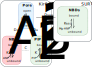
\includegraphics[width=0.7\textwidth]{regulation_diagram.pdf}
	\caption[Modes of regulation of K\ATP{} - reprinted]{
	Adapted from \cite{puljung_cryo-electron_2018}, duplicated from Figure \ref{ch1fig:regulation_diagram}.
	The open-closed equilibrium of the K\ATP{} channel pore (denoted as $L$) is energetically coupled to three different ligand binding sites.
	The four inhibitory nucleotide binding sites of Kir6.2 bind either ATP or ADP (generalised to ANP) with an equilbrium binding constant $K_A$.
	The four stimulatory PIP\textsubscript{2} binding sites of Kir6.2 bind PIP\textsubscript{2} with an equilbrium binding constant $K_B$.
	The four stimulatory Mg-nucleotide binding sites formed by the dimerisation of the NBDs of SUR1 (labelled as NBDs) bind either ATP or ADP with an equilbrium binding constant $K_C$, and Mg\textsuperscript{2+} is required for transduction.
	Each binding domain interacts with the channel pore according to the factors $D_A$, $D_B$, and $D_{NBD}$ respectively.
	In addition, there is a potential coupling between the inhibitory nucleotide binding site of Kir6.2 and the stimulatory PIP\textsubscript{2} binding site of Kir6.2 described by the factor $C$.
	}\label{ch7fig:regulation_diagram}
\end{figure}

How does inhibitory nucleotide binding to Kir6.2 interplay with the stimulatory nucleotide binding to the NBDs of SUR1?
In parallel work published in \textcite{puljung_activation_2019-1}, we established a similar experimental paradigm to measure MgTNP-ADP binding to NBS2 of SUR1 in unroofed membranes.
While we were unable to measure current activation and nucleotide binding simultaneously, we collected data separately for the two processes.
Here we refit that data in combination with the inhibition data presented in Figure \ref{ch3fig:pcf_1}to an MWC model which comprises both inhibition at Kir6.2 by TNP-ATP and activation at SUR1 by MgTNP-ADP with a shared open probability (Figure \ref{ch7fig:activation_fits}).
Comparison of the binding association constants for TNP-nucleotides at Kir6.2 and NBS2 shows that MgTNP-ADP binds more readily to NBS2 than TNP-ATP binds to Kir6.2 (Figure \ref{ch7fig:activation_params_1}).
In contrast, the transduction of binding is far stronger for TNP-ATP bound to Kir6.2 than for MgTNP-ADP bound to NBS2.
In terms of free energy, binding to Kir6.2 contributes \SIrange{32.7}{68.0}{\kilo\joule\per\Molar} to the closed state of the channel(slightly higher than the \SIrange{23.0}{63.4}{\kilo\joule\per\Molar} estimated from fitting the inhibition data alone), whereas binding to NBS2 contributes \SIrange{0.6}{33.9}{\kilo\joule\per\Molar} to the open state of the channel.

\begin{figure}[hbtp]
	\centering
	\begin{subfigure}[t]{0.9\textwidth}
		\caption{}\label{ch7fig:activation_fit_1}
		\centering
		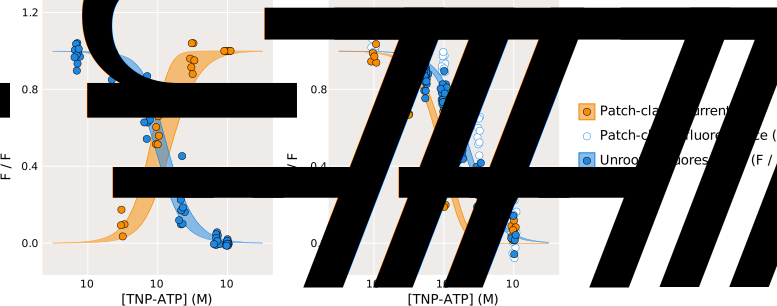
\includegraphics[width=\textwidth]{activation_fit_1.pdf}
	\end{subfigure}
	\vfill
	\begin{subfigure}[t]{0.9\textwidth}
		\caption{}\label{ch7fig:activation_params_1}
		\centering
		
\includegraphics[width=\textwidth]{activation_params_1.pdf}
	\end{subfigure}
	\caption[TNP-ATP inhibits K\ATP{} more strongly than MgTNP-ADP activates it]{
	\subref{ch7fig:activation_fit_1} Fluorescence quenching (blue) and current inhibition (orange) of W311*-GFP+SUR1 by TNP-ATP (left) or fluorescence quenching (blue) and current activation (orange) of G334D+SUR1-T1397* by MgTNP-ADP (right).
	The fluorescence quenching data shown here are from unroofed membranes.
	Activation data are reproduced from \textcite{puljung_activation_2019-1}, inhibition data from Figure \ref{ch3fig:pcf_1}.
	Fitted curves are the median estimate (lines) and the \SI{95}{\percent} credible intervals (shaded areas) of the posterior probability distribution of fits to the MWC model parameterised in equations \ref{eq:mwc_binding} and \ref{eq:normalised_po}, not including the $\delta_{experiment}$.
	\subref{ch7fig:activation_params_1} Posterior probability distributions for each of the five free parameters estimated from fits to the MWC model are shown shaded according to their credible intervals.
	$1/D_{NBD}$ is plotted to aid comparison with $D_A$.
	}\label{ch7fig:activation_fits}
\end{figure}

Assuming that the excitatory and inhibitory processes are independent, inhibition would be expected to dominate under conditions at which all the nucleotide binding sites of K\ATP{} are occupied.
This is consistent with published measurements of wild-type KATP in the presence of Mg\textsuperscript{2+} \cite{proks_activation_2010}.
The ability of MgADP to increase K\ATP{} currents in the presence of ATP \cite{gribble_mgatp_1998-1} and the bell-shaped MgADP concentration response curve for K\ATP{} \cite{proks_activation_2010, vedovato_nucleotide-binding_2015} can then be explained by the higher binding affinity of NBS2 resulting in an increase in current at low nucleotide concentrations, followed by inhibition at higher concentrations due to stronger transduction from nucleotides binding to Kir6.2.

Of course, this interpretation relies on data which has been obtained from different constructs and under different conditions.
Ideally, we would explore this further by carrying out patch-clamp fluorometry experiments under conditions where all three nucleotide binding sites simultaneously affect channel gating (in the presence of Mg\textsuperscript{2+}).
Our initial attempts to do so were limited by the rapid rate of rundown of K\ATP{} currents in the presence of divalent ions, which made it difficult to collect useable data with simultaneous current and fluorescence recordings.
Introducing mutations which slow the rate of rundown may be one method to ameliorate this problem and synthesise a more complete model of K\ATP{} function.

How does inhibitory nucleotide binding to Kir6.2 interplay with PIP\textsubscript{2} regulation of the K\ATP{} channel?
As descibed in Chapter \ref{ch:1-intro}, directly measuring or varying the PIP\textsubscript{2} concentration in the membrane is challenging, and in the experiments presented here we have tried as far as possible to keep PIP\textsubscript{2} constant.
Our simplifying assumption which assumes PIP\textsubscript{2} acts solely on the open probability of the channel and does not vary significantly in our recordings seem sufficient to explain the variety of effects we see from the mutations studied in Kir6.2 and SUR1.

However, it remains an open question as to whether PIP\textsubscript{2} binding to Kir6.2 only affects the channel through increasing the open probability (Figure \ref{ch7fig:regulation_diagram}, $D_B$) or whether there is a mechanism which directly couples the PIP\textsubscript{2} binding site to the inhibitory nucleotide binding site (Figure \ref{ch7fig:regulation_diagram}, $C$).
Our experiments with substitutions at E179 on Kir6.2, predicted to be in the PIP\textsubscript{2} binding pocket, do not rule out the existence of a direct coupling.
However, the observed reduction in the binding affinity for TNP-ATP is only circumstantial evidence as it may also be explained by the two substitutions examined (E179A and E179K) altering the nucleotide binding pocket instead.
Experiments to directly test for the existence of direct coupling would need to involve manipulation and measurement of PIP\textsubscript{2} levels.

\section{Nucleotide inhibition of the K\ATP{} channel in the context of other ligand-gated ion channels}

The K\ATP{} channel is one of many ion channels regulated by ligands.
The MWC model used here to fit TNP-ATP inhibition of K\ATP{} allows us to compare nucleotide regulation of the K\ATP{} channel to other ion channels which are well described by such models.
One particularly well studied channel is the nicotinic acetylcholine receptor (nAChR).
The binding of acetlycholine (ACh) to the nAchR increases the open probability of the channel in a similar fashion as the binding of nucleotides to Kir6.2 decreases the open probability of the K\ATP{} channel.
\textcite{auerbach_thinking_2012} estimated that the transduction energy which saturating concentrations of ACh contribute to the open state of the nAChR is approximately \SI{25}{\kilo\joule\per\Molar}, remarkably similar to the \SIrange{23.0}{63.4}{\kilo\joule\per\Molar} we estimate saturating concentrations of TNP-ATP contribute to the closed state of the K\ATP{} channel.
Similarly, \textcite{horrigan_coupling_2002} characterised the regulation of the large conductance K\textsuperscript{+} (BK) channel by voltage and Ca\textsuperscript{2+} using an MWC framework, and estimated a transduction energy of approximately \SI{21}{\kilo\joule\per\Molar} in favour of the open state at saturating Ca\textsuperscript{2+} concentrations.
As a final comparison, \textcite{varnum_subunit_1996} investigated the regulation of the cyclic-nucleotide gated (CNG) channel by cGMP, cIMP and cAMP and estimated transduction energies of \SI{34}{\kilo\joule\per\Molar}, \SI{29}{\kilo\joule\per\Molar}, and \SI{15}{\kilo\joule\per\Molar} to the open state respectively.
It appears that the energy ligand binding contributes to conformational change is broadly similar across diverse ion channel families regulated by structurally dissimilar ligands.

Moving forwards, it would be particular interesting to apply similar binding assays and MWC functional modelling to other ATP-regulated ion channels such as the P2X receptor family \cite{khakh_p2x_2006}.
While K\ATP{} channels are inhibited by intracellular ATP, the P2X receptor family are axctivated by extracellular ATP, and differences in the ATP concentrations and dynamics in these two spaces suggest there may be other biophysical differences in nucleotide regulation, upon which direct measurements of nucleotide binding may be able to shed light \cite{mansoor_x-ray_2016}.
